%BEGIN: DiaSim 
\section{DiaSim: A Parameterized Simulator for Pervasive Computing Applications}\label{sec:diasim}

DiaSim is a Java based simulator for pervasive computing applications based on sensors and actuators \cite{bruneau2013diasim}. In this project, the simulation process starts out by defining a high-level description of the target pervasive computing environment, in a domain specific language: DiaSpec. Part of this definition are \emph{classes of entities} and \emph{data types} which can be exchanged by the entities. Based on this definition, DiaGen produces a customized \emph{programming framework} and an \emph{emulation layer}.\\

\begin{figure}[H]
	\centering
	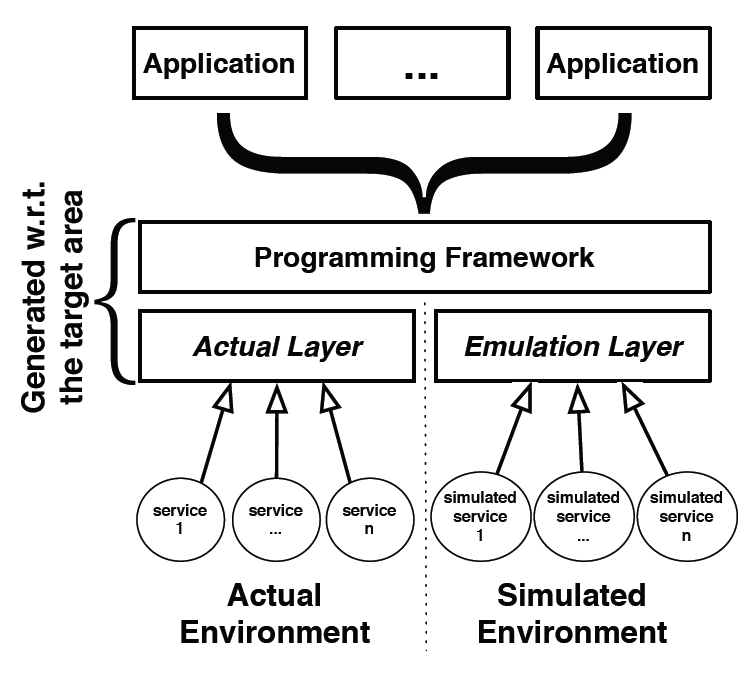
\includegraphics[width=\linewidth]{gfx/Chapter2/diasim_layered_architecture}
	\caption{DiaSim layered architecture}
	\label{fig:diasim_architecture}
\end{figure}

As depicted in Figure \ref{fig:diasim_architecture}, the simulator has a modular, layered architecture. Applications written using the generated programming framework, can be run both in a simulated and a real-world environment. In the real environment, the data comes from real sensors, while in the simulated environment the data comes from simulated sensors in the emulation environment. Besides the components mentioned so far, DiaSim also includes a simulation renderer, enabling the researcher to visually monitor and debug the pervasive computing system.\\

At the heart of this simulator, they have built simulation model. The core entity is called a \emph{stimuli}. This represents changes of the environment observable by the sensors in the system. Entities that generate stimuli are called \emph{stimulus producers}, producing only one type of \emph{stimulus}. The generated stimuli may trigger sensors (e.g. a motion detector) which publish events, that may in turn stimulate actuators or services. Hence, we can see a stimuli as a type of stimulus; making an analogy in object-oriented programming, stimulus would be a class, stimuli would be an instance of that class and the stimulus producer would be a factory \cite{gamma1994design}, producing instances of the stimulus class based on a certain set of rules. These rules define the evolution of the stimuli in terms of space, time and intensity (e.g. an agent moving from one location to another). Each stimulus has a type associated with it, matching the type one at least one sensor in the system.\\

\begin{figure}[H]
	\centering
	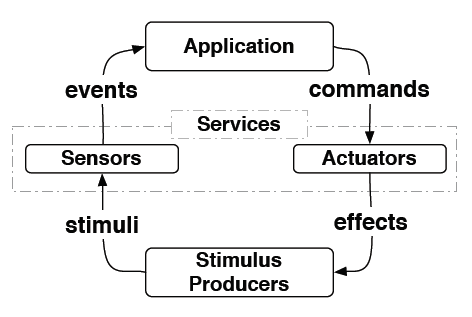
\includegraphics[width=\linewidth]{gfx/Chapter2/diasim_simulation_model}
	\caption{DiaSim simulation model}
	\label{fig:diasim_simulation_model}
\end{figure}

As illustrated in Figure \ref{fig:diasim_simulation_model}, besides stimulus producers, the simulated environment also contains simulated services; they process stimuli, perform actions and interact with other services. The two key services in this simulator are \emph{sensors} and \emph{actuators}. The interaction between services and the environment are based on one of the existing three interaction modes:
\begin{itemize}
	\item Command (one-to-one, synchronous interaction). Usually received by actuators to modify their state (e.g. on/off command for a light)
	\item Event (one-to-many, asynchronous interaction). Usually generated by sensors when they receive stimuli (e.g. a motion detector when receiving location stimuli matching its room, would generate an event containing the room's number)
	\item Session (one-to-one with information exchange over a period of time). For example, when motion from an unknown source is detected in a restricted area, an audio notification service could stream a warning audio notification to a nearby speaker service.
\end{itemize}

\subsection{Siafu}\label{sub:siafu}
To render the simulation, DiaSim was coupled with Siafu \cite{siafu:online}, a highly customizable, open-source Java based simulator for mobile context-aware applications and services \cite{martin2006generic}.\\

Siafu was meant to be a flexible simulator. Hence, they have separated the main information sources from each other:
\begin{itemize}
	\item Agent Model. Takes decision on what a certain agent should do given it's current context and the status of surrounding entires. As a result, the model will change the properties of an agent (e.g. standing, sitting, walking etc.). A special property is the destination. This will make the agent move in the surrounding environment; movement and path finding routines are handled automatically by the simulator.
	\item World Model. Consists of an environment model, places of interest (e.g. office, rooms etc.) and global events model (e.g. holidays, happy hour at a restaurant etc.)
	\item Context Model. Manages context variables used in the simulation.
\end{itemize}

The simulated data is available in 2D graphical representation and through a web service interface.\\
%END: DiaSim 